
\documentclass{beamer}

\usepackage[T1]{fontenc}
\usepackage[utf8]{inputenc}
\usepackage[french,english]{babel}

\usepackage{lmodern}
\usepackage{amsthm}
\usepackage{float}
\usepackage{lmodern}%pour un meilleur rendu des polices
\usepackage{verbatim}%du texte non interprt
\usepackage{amsmath}
\usepackage{amssymb}%maths
\usepackage{xspace}
\usepackage[dvipsnames,svgnames,table]{xcolor}
\usepackage{listings}
\usepackage{fancyhdr}
\usepackage{etoolbox}
\usepackage{titlesec}
\usepackage{titletoc}
\usepackage{lastpage}
\usepackage{hyperref}
\usepackage{ctable} % for \specialrule command
\usepackage{cite}
\usepackage{algorithm2e}
\usepackage{alltt}
\usepackage{array}
\usepackage{mdwmath}
\usepackage{mdwtab}
\usepackage{eqparbox}
\usepackage{subfig}
\usepackage{dblfloatfix}
\usepackage{url}
\usepackage{tipa}
\usepackage{stmaryrd}
\usepackage{upgreek}
\usepackage{mathrsfs}
\usepackage{ulem}
\usepackage{cancel}

\graphicspath{{img/}}
\DeclareGraphicsExtensions{.pdf,.jpeg,.jpg,.png}


\newcommand{\ccite}[1]{\textbf{\cite{#1}}}
\newcommand{\pd}[2]{\dfrac{\partial #1}{\partial #2}}
\newcommand{\od}[2]{\dfrac{\mathscr{D}_a #1}{\mathscr{D} #2}}
\newcommand{\tensor}[1]{\mathbf{#1}}
\renewcommand{\vector}[1]{\overrightarrow{#1}}

\newcommand{\Tau}{\tensor{\mathlarger{\uptau}}}
\renewcommand{\v}{\vector{u}}
\newcommand{\W}{\tensor{W\left( \v \right)}}
\newcommand{\D}{\tensor{D\left( \v \right)}}
\newcommand{\grad}{\vector{\nabla}}
\newcommand{\gradv}{\tensor{\nabla\v}}
\renewcommand{\div}[1]{div \left( #1 \right)}
\newcommand{\divv}[1]{\vector{div} \left( #1 \right)}
\newcommand{\UU}{\mathcal{U}}
\newcommand{\VV}{\mathcal{U}}
\newcommand{\M}{\mathcal{M}}
\newcommand{\A}[2]{\mathcal{A}_{#1}\left( #2 \right)}
\newcommand{\Uu}{\UU^{n}}
\newcommand{\Uv}{\UU^{n+\theta}}
\newcommand{\Uw}{\UU^{n+1-\theta}}
\newcommand{\Ux}{\UU^{n+1}}
\newcommand{\Uk}{\UU^{k}}
\newcommand{\Ukk}{\UU^{k+1}}
\newcommand{\Vk}{\VV^{k}}
\newcommand{\Vkk}{\VV^{k+1}}
\newcommand{\Tauk}{\Tau^{k+1}}
\newcommand{\vk}{\v^{k+1}}
\newcommand{\pk}{p^{k+1}}
\newcommand{\Dk}{\tensor{D\left( \vk \right)}}

\definecolor{lightgray}{gray}{0.9}
\definecolor{titlecolor}{RGB}{0,0,200}
\definecolor{subtitlecolor}{RGB}{0,0,153}
\definecolor{textcolor}{RGB}{0,128,255}
\definecolor{RoyalPurple}{RGB}{102,51,153}
\definecolor{ForestGreen}{RGB}{34,139,34}


\newcommand{\colbox}[1]{\colorbox{lightgray}{$ #1 $}}

\newcommand{\stitle}[2][0.3cm] { 
    {\normalsize \textcolor{titlecolor}{\textbf{#2}}} 
    \vspace{#1} 
}

\newcommand{\ssubtitle}[1]{ {\footnotesize \textcolor{subtitlecolor}{\textbf{#1}}} }

\newcommand{\stress}[1]{\textcolor{textcolor}{#1}}

\newcommand{\hidecontent}[2][0.25]{{% \hidecontent[<transparency>]{<stuff>}
  \setbox9=\hbox{#2}% Store <stuff> in \box9 to obtain height/width
  \transparent{#1}\ooalign{\usebox9\cr\color{white}\rule{\wd9}{\ht9}\cr}}}


\begin{document} 

\maketitle 

\section{Introduction}

This paper,
published in 2009 by Marc Honnorat,
Jerome Monnier and François-Xavier Le Dimet,
proposes a method to combine Eulerian and Lagrangian data from remote sensing observations in a variational framework for a river hydraulics model based on the 2D shallow water equations.
In addition to classical height sensors that provides sparse Eulerian observations,
physical particles are dropped into the fluid and advected by the flow.
Their trajectories is then extracted from video images using image extraction techniques (image velocimetry).
This additional Lagrangian data provides information on the surface velocity thanks to an appropriate transport model.
It is demonstrated that this method allows significant improvements in the identification of local bed elevation,
as well as initial conditions through numerical twin assimilation experiments.
At the time of publication of this paper,
no physical prototype was built and thus the problem of trajectory extraction was not tackled.


\section{Shallow Water Model}

The numerical simulation of river flows requires a precise modelling of the underlying physics and the bidimentional shallow water equations can describe accurately many free surface hydraulic configurations.

\vskip 0.3cm
With $\u(x,y,t)$ the depth averaged velocity vector, $\h(x,y,t)$ the height of the free surface, $\q = \h\u$ the local discharge, $\n(y)$ the Manning roughness coefficient, $\zb(x,y)$ the bed elevation,  this model can be written as the following :

$$
\begin{equation}
\colbox{
\label{shallow}
\left\{
\begin{array}{l l l c r l l}
    \multicolumn{5}{l}{\pd{\h}{t} + div(\q)} 
    &=& 0 \\
    \multicolumn{5}{l}{\pd{\q}{t} + \div(\u \times \q) + \frac{1}{2} \g \grad \h^2 + \g\h\grad\z + \g\frac{\n^2 \norm{\q}}{\h^{\frac{7}{3}}}\q}
    & = & \vecbf{0} \\
    \h(t=0) & = & \hz && \q(t=0) & = & \qz \\ 
    (\q \cdot \nv)_{|\gq} & = & - \qb &&
    (\q \cdot \nv)_{|\gw} & = & 0 \\
    (\nabla \q \times \nv)_{|\gt}  & = & \vecbf{0} &&
    (\grad \h \cdot \nv)_{|\gq \cup \gw \cup \gt}  & = & 0 \\
    \h_{|\gz} & = & \zs - \zb_{|\gz} &&
    \grad(\u \cdot \nv + 2c) \cdot \nv & = & 0 \\
    \multicolumn{7}{l}{c = \sqrt{2\g\h} \equationrm{\ \ \ \ (local\ wave\ celerity)}}
\end{array}
\right.
}
\end{equation}
$$

The domain boundary $\partial \Omega = \Gamma$ is split into four boundaries $\gq \cup \gz \cup \gt \cup \gw$ which correspond to open boundaries for the 3 first ones and walls for the last one.
$\gz = \{ y \in \R\ |\ \u(x_{max},y) \cdot \nv > 0 \}$ is the downstream boundary where a water elevation $\zs$ should be specified for subcritical flows $\norm{\u} < c$.
Here $\Omega$ is a box $\left[0,x_{max}=100m \right] \times \left[ 0,y_{max}=16m \right] \times \left[ 0, z_{max} = 1.2m \right]$ with features a 0.4\% slope on the $x$-axis with an additional bump which can be seen in figure~\ref{domain} page~\pageref{domain}.

\vskip 0.3cm
The problem is that in order to carry out a realistic simulation this numerical model requires information on physical parameters such as the bed elevation $\zb$,
roughness coefficients $\n$ in addition to initial conditions $\hz$ and $\uz$ which are usually not well known.
Since the quality of the simulation is largely dependant on those model inputs,
those must be defined accurately and thus we try to identify them with data assimilation.

\vskip 0.3cm
Initial conditions and boundary conditions can be gathered in the control vector $\k = (\hz, \qz, \n, \zb, \qb, \zs)$ but in the paper they fix $n$ to a known piecewise linear function, $\qb$ to constant discharge $8m^3/s$, and $\zs \simeq 0.4m$ so the real control vector is rather $\k = (\hz, \qz, \zb)$.

\clearpage

\begin{figure}[H]
   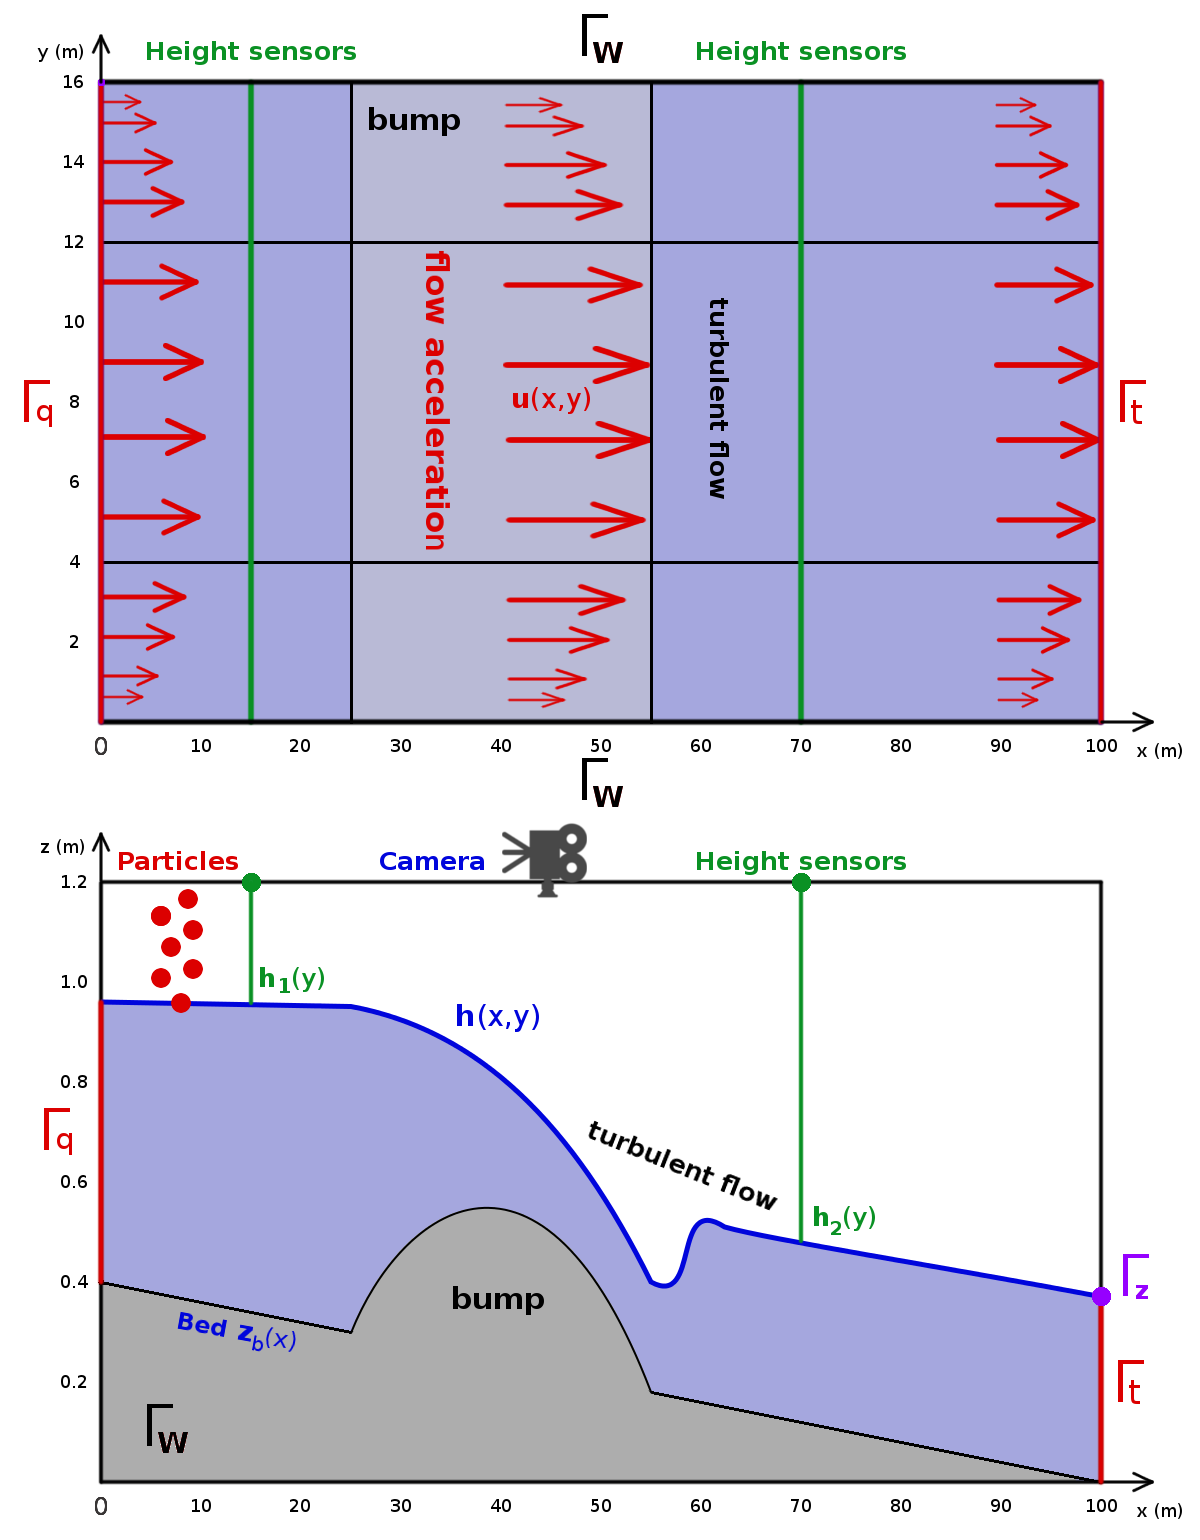
\includegraphics[width=16cm]{domain2}
   \caption{\label{domain} 
       Description of the domain $\Omega$ (top and side view) and illustration of the proposed method.
       Height sensors are recording the height of the free surface over the whole width $[0,y_{max}]$ of the domain at $x=15m$ and $x=70m$ which brings classical Eulerian observations for the data assimilation process.
       In addition to this, 32 particles are uniformly dropped every $p \Delta T = 2s$ at $x=10m$ over the whole width of the domain, their trajectories are captured and are than extracted from video recording which brings Lagrangian data.
}
\end{figure}

\section{Lagrangian Data Assimilation}

The proposed method is described in figure~\ref{domain} page~\pageref{domain}.
In order to use such Lagrangian data,
a link must be made between the Shallow Water model and a model describing particle movement advected by the flow.
For each particle $P_i$ entering the domain at $t=t_i^0$ and leaving at $t=t_i^f$,
a simple transport model can describe its trajectory $\Xi(t)$ with depth averaged velocity $\u$ :

$$
\begin{equation}
\colbox{
\label{transport}
\left\{
\begin{array}{l c l}
    \fd{\Xi}{t}(t) &=& \v(\Xi(t), t) \\
    \Xi(t_0^i) &=& \mathbf{x}_0^i \\
    \v &=& \gamma \u\ \ \gamma \in\ ]0,1]
\end{array}
\right.
}
\end{equation}
$$

This model is weakly coupled with equations ($\ref{shallow}$).
Because the Shallow Water model does not take into account physical perturbations of the water surface,
a low pass filter should be applied to remove small scale perturbations of the Lagrangian dataset.
This is based on the \textit{a priori} information that the flow is in a steady state.
Instead of considering the $N_{obs}$ trajectories $\Xi(t)$ extracted from video,
we seek to create a set of $N_m$ filtered trajectories $\Xj(t)$,  
with synchronised starting time and uniformly sampled initial positions $(t^j_0, \mathbf{x}^j_0) \in p\Delta T\ \mathbb{Z} \cap [0,T] \times \{x=10m\} \times [0,y_{max}]$. 

\vskip 0.3cm
Those filtered trajectories $\Xj$ satisfy $\eqref{transport}$ with a mean velocity $\vb_j(t) = \v(\Xj(t), t)$ defined by a local spacial and temporal average on a time-space window $\W_j(t) = \Wt \times \Wx \subset [0,T] \times \Omega$ of the observed trajectories $\Xi$. More precisely we define $\vb_j$ as :

$$
\begin{equation}
\label{filter}
\colbox{
\left\{
\begin{array}{l c l}
    \vb_j(t) &=& \dfrac{1}{\sw_j(t)} \displaystyle \sum_{i = 1}^{N_{obs}} \int_0^T \fd{\Xi(s)}{s} \I_{\Wt(t)}(s) \I_{\Wx}(\Xi(s)) \ds \\
    \sw_j(t) &=& \displaystyle \sum_{i = 1}^{N_{obs}} \int_0^T \I_{\Wt(t)}(s) \I_{\Wx}(\Xi(s)) \ds \\
\end{array}
\right.
}
\end{equation}
$$

Now that the link between Lagrangian data and Eulerian data has been made, the data assimilation framework is a classical one. We want to minimize the following cost function :

$$
\colbox{
\J(\k) =  
\J(\hz, \qz, \zb)
}
$$
$$
\colbox{
= \underbrace{\displaystyle \dfrac{1}{2} \sum_{i=1}^{2}\int_0^T \int_0^{y_{max}} \left[ h(x_i,y) - h_i^{obs}(y) \right]^2 \dy \dt}_{\mathrm{water\ depth\ discrepancy}}
+ \underbrace{\displaystyle \dfrac{\alpha_t}{2} \sum_{j=0}^{N_m} \int_0^T \norm{\X_j(t) - \Xj(t) }^2 \dt}_{\mathrm{filtered\ trajectories\ discrepancy}}
+ \underbrace{\displaystyle \dfrac{\alpha_p}{2} \iint_{\Omega_{xy}} \norm{\grad \zb(x,y)}^2 \dx \dy}_{\mathrm{topography\ regularization\ term}}
}
$$

A bed regularization term is included to prevent topography explosions (we want to penalize abrupt variations of the bed).

\clearpage
\section{Twin experiments}

\subsection{Simulation}

The effectiveness of this new method is only demonstrated with twin experiments with the help of Dassflow,
a software designed to carry out data assimilation experiments.
The discretization of the direct Shallow Water model ($\ref{shallow}$) relies on finite volume method and the HLLC approximate Riemann solver included in Dassflow.
The adjoint model is directly obtained with the automatic differentiation tool Tapenade.
The weakly coupled transport model (\ref{transport}) is solved with $\gamma = 1$ using a second order Runge-Kutta scheme and Q1-Lagrange interpolation on the piecewise velocity field $\u$ solution of ($\ref{shallow}$).
A total of $N_m = 200$ virtual trajectories $\X_j$ are integrated using RK2 by dropping 10 virtual particles every $p\Delta T = 2s$ into the flow uniformly at $x=10m$.
Here there is no need for trajectory filtering because the model already do this for us (neither (\ref{shallow}) nor (\ref{transport}) does take into account small scale perturbations).


\vskip 0.3cm
Twin data assimilation experiments are carried out for a simulation time $T = 100s$ and constant time step $\Delta T = 0.1s$. It is not clear whether they take into account inevitable transient flow or not because they only generate particle trajectories up to $t = 40s$ and that is pretty incoherent with what they claim (no reason to stop the generation before the end of the simulation, unless they only want full trajectories which would impose a maximal particle mean velocity of $100m/min$).
Reference initial conditions $\k^{ref}$ are taken as steady state of a simulation where the slope $\zb$ features the bump.
We seek to identify the reference bed elevation $\zb$ and reference initial conditions $\uz$ and $\qz$ with following initial guess :
initial conditions $\k_0$ are taken as steady state of the same simulation where the slope $\zb$ is linear ($ie.$ without the bump).

\subsection{Data generation}

Because there is only Twin experiments, all observations are generated from the models.
Height observations are perfect and continuously recorded during time using the given initial condition.

\vskip 0.3cm
A set of $N_{obs} = 640$ trajectories $\X_i^{obs}$ are perfectly observed by uniformly dropping $32$ particles every $p\Delta T = 2s$ at $x = 10m$ in a turbulent velocity flow $\mathbf{v}^{tr} = \v + \mathbf{\tilde{v}}$ where $\mathbf{\tilde{v}}$ is a Gauss-Markov zero-mean stochastic process which act as turbulences. 
Those particles are then filtered using $(\ref{filter})$. A total of $N_m = 200$ filtered trajectories $\Xj$ are obtained by taking the same initial space and time conditions as the reference ones $\X_j$. Here they took the following integration support centered on the filtered particle $\W_c(t) = [0,T] \times [0,1m] \times [0,1m]$ because it has been found as being a good compromise.


\clearpage

\section{Results}
\subsection{Bed identification}
    
Here we only look for bed elevation $\zb$ and $\uz$ and $\qz$ are fixed.
They show through their twin experiments that bed identification is not possible when using only height informations. 
Trying to use particle data without filtering it shows little improvements but the bed features many small scale variations of large amplitude.
When using the filtered particles as observations, they expose substantial improvement in the quality of identification.

\subsection{Joint identification}
    
Here we look for bed elevation $\zb$ as well as initial conditions $\uz$ and $\qz$.
With filtered particles as observations the results are still satisfactory for the bed elevation $\zb$ but initial condition identification for the velocity $\uz$ is not amazing. The identification of $\qz$ is a bit better but features large variations between $x=0m$ and $x=20m$.

\section{Conclusion}

In this paper was presented a novel theoretical method to include Lagrangian data observation into a variational framework to improve the identification of control variables like the bed elevation of a river. The link between Eulerian and Lagrangian observations is made via a weakly coupled transport model. A spatio-temporal filter has been introduced to extract meaningful data with respect the Shallow Water model from the observed particles which are subject to small-scale perturbations, improving the identification. To further restrict the dimensions of the control space, a regularization term was introduced to keep the bed elevation with a smooth profile and penalize large variations. 

\end{document}




 
 
 
 
 
 
 
 
 
 
 
 
